\documentclass[a4paper,11pt]{article}

\usepackage[english]{babel}
\usepackage{xltxtra}
\usepackage{alltt}
\usepackage[backend=bibtex]{biblatex}
\usepackage{listings}
\usepackage[usenames,dvipsnames]{color}
\usepackage{hyperref}
\usepackage{float}

\bibliography{references}

%
% Some initialization stuff.
%

% Custom title command with subtitle support.
\newcommand{\Title}[2]{\title{#1\\\textsc{\large #2}}}

\hypersetup{
    % Disable red boxes around hyperlinks.
    pdfborder = {0 0 0}
}

\lstset{
    % Settings for listings package.
    language=Java,
    frame=single,
    frameround=tttt,
    xleftmargin=2.5em,
    xrightmargin=2em,
    basicstyle=\ttfamily,
    showstringspaces=false,
    captionpos=b,
    aboveskip=1.5em,
    belowcaptionskip=0pt,
    belowskip=1em,
    numbers=left,
    numberstyle=\ttfamily\color{Gray}
}

\Title{MiniJava Compiler (\texttt{mjc})}{DD2488 -- Project Report}

\date{XX May 2014}

\author{Daniel Månsson\\dmans@kth.se \and Elvis Stansvik\\stansvik@kth.se}

\begin{document}

\maketitle

\begin{abstract}
\noindent In this brief report we introduce \texttt{mjc}, a compiler for the MiniJava
language targeting the Java Virtual Machine (JVM). The compiler was built as part of
the course \emph{DD2488 Compiler Construction} at KTH. We begin the report with a description
of the compiler design, followed by instructions for building and running the compiler,
and conclude with some thoughts on possible future improvements.
\end{abstract}

\tableofcontents

\thispagestyle{empty}

\newpage

\section{Introduction}

MiniJava is a subset of the Java programming language presented in \cite{appel}
\footnote{Not exactly true: A Java compiler checks that variables are initialized before
use, while in MiniJava this is simply undefined run-time behavior.} The original language
supports the built-in types \texttt{int}, \texttt{int[]} and \texttt{boolean} as well as
user defined class types. There is no support for inheritance or method overloading.
Operators \texttt{+}, \texttt{-}, \texttt{*} and \texttt{<} are defined on integers.
Operators \texttt{\&\&} and \texttt{!} are defined on booleans.

\texttt{mjc} is a compiler for a slightly modified and extended version of MiniJava
\cite{grammar}, adding support for operators \texttt{<=}, \texttt{>}, \texttt{>=}
on integers; operators \texttt{==} and \texttt{!=} on integers, booleans and
references; operator \texttt{||} on booleans; \texttt{if} statements
without an \texttt{else} clause; array bounds checks and nested blocks with new variable
declarations. The compiler targets the Java Virtual Machine (JVM) by producing
Jasmin \cite{jasmin} pseudo-assembly code as output.

We begin this report with an overview of the design of \texttt{mcj}, followed by some
instructions for building and running the compiler. We conclude with some thoughts on
possible future improvements.

\section{Compiler Design}

\label{sec:design}

The compilation process in \texttt{mjc} proceeds in four phases. The process begins with
the input of MiniJava source code and ends with the output of Jasmin assembly code.
Each intermediate phase takes its input from the preceding phase and gives as
output the input for the next. Figure~\ref{fig:compiler_phases} shows an illustration
of the compilation phases.

\begin{figure}[h!]
    \centering
    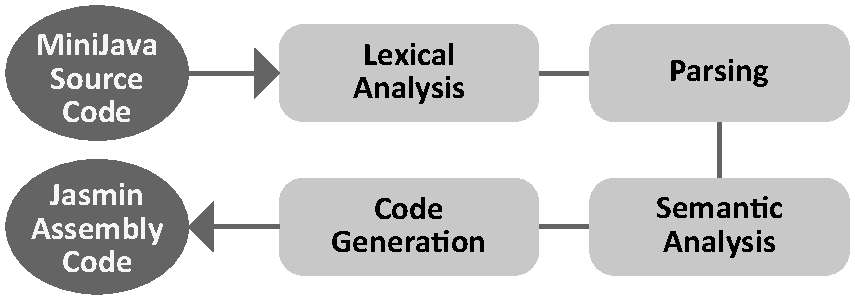
\includegraphics[width=0.8\linewidth]{figures/compiler_phases.pdf}
    \caption{Compilation phases in \texttt{mjc}.}
    \label{fig:compiler_phases}
\end{figure}

In the following subsections, we'll briefly go through each compilation phase and
explain it in general terms. We'll also explain design decisions we made and any
challenges we faced in constructing \texttt{mjc}.

\subsection{Lexical Analysis and Parsing}

Compilation begins by breaking the input byte stream into a stream of terminal
symbols (tokens) and parsing the resulting token stream into an abstract syntax
tree (AST). The lexical analyzer (lexer) must check that the input consists of
valid MiniJava tokens. The parser must check that the resulting token stream is
part of the formal language described by the MiniJava grammar.

We decided to use the SableCC \cite{sablecc} parser generator for lexical analysis
and parsing in \texttt{mjc}. SableCC takes as input a file containing a set of
regular expressions describing valid tokens, and an LALR grammar describing the
input language. The output is a complete lexer and parser, along with some abstract
visitor classes for traversing the AST.

Codifying the provided MiniJava grammar as a SableCC input file was fairly
straightforward. To simplify later stages of compilation, a depth first traversal
of the AST should correspond to the precedence rules of MiniJava operators. This
took some careful composition of the productions for expressions.

We also wanted the parser to reject input such as \lstinline{new int x[2][1]}
instead of interpreting it as the creation of an integer array followed by an
access of its second element. To accomplish this we had to introduce an additional
production for primary expressions, one that excluded array creation expressions,
and use that in the production for array accesses.

\subsection{Semantic Analysis}

Past lexical analysis and parsing, we know that the input program is lexically and
syntactically correct. But other errors such as uses of undeclared identifiers
and type errors may still exist in the program. During semantic analysis, the
compiler traverses the AST looking for such errors.

\begin{figure}[h!]
    \centering
    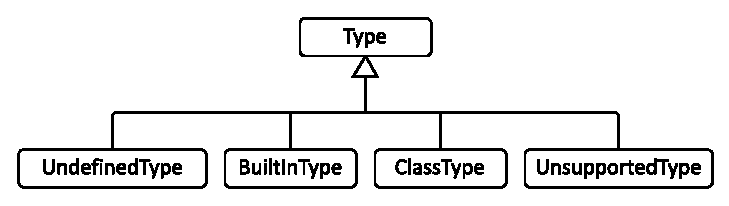
\includegraphics[scale=0.9]{figures/type_classes.pdf}
    \caption{Type class hierarchy.}
    \label{fig:type_classes}
\end{figure}

To represent built-in types \texttt{int}, \texttt{int[]} and \texttt{boolean} as
well as user defined class types, we came up with the class hierarchy shown in
figure~\ref{fig:type_classes}. The abstract base class \texttt{Type} specifies
methods such as \texttt{isAddableTo(Type)} to be implemented by subclasses. Each
of \texttt{int}, \texttt{int[]} and \texttt{boolean} is represented by a static
instance of \texttt{BuiltInType}. \texttt{UnsupportedType} is used for the
\texttt{void} and \texttt{String[]} ``types''. These exist grammatically in
MiniJava but lack meaningful semantics. \texttt{UndefinedType} will be explained
shortly.

\begin{figure}[h!]
    \centering
    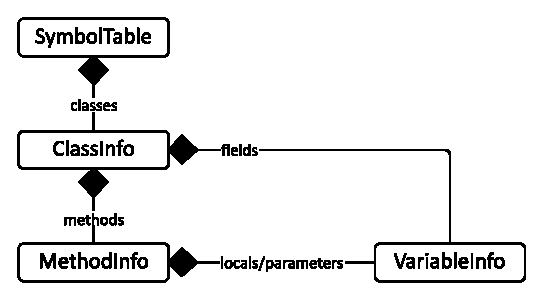
\includegraphics[scale=0.9]{figures/symbol_table_classes.pdf}
    \caption{Symbol table class composition.}
    \label{fig:symbol_table_classes}
\end{figure}

Semantic analysis begins with the construction of a \emph{symbol table}. For
each class name, method name and identifier found in the program, the symbol table
stores information such as the name and type of the symbol as well as the source
code location where it was declared. Figure~\ref{fig:symbol_table_classes} shows the
composition of the classes we used to represent the symbol table.

\texttt{MethodInfo} deserves some special mention. To handle the adding and look-up of
local variables, which may be declared in nested blocks, \texttt{MethodInfo} has
an \texttt{enterBlock()/leaveBlock()} API which is used in conjunction with
\texttt{addLocal(..)}/\texttt{getLocal(..)} to control the scoping of local variables.

Local variables are kept in a multimap, since two variables may have the same name if
the block in which the first one is declared is closed at the point of the second
declaration. Blocks inside a method are numbered $0, 1, \ldots$ in the order in which
they are opened. Internally \texttt{MethodInfo} maintains a stack of currently
open blocks. \texttt{enterBlock()} pushes the next block (taken from a counter) on
the stack, while \texttt{leaveBlock()} pops the stack.

Each \texttt{VariableInfo} holds the number of the block in which the variable
was declared. \texttt{addLocal(..)} sets the block number of the added
\texttt{VariableInfo} to the current block (top of the stack). \texttt{getLocal(..)}
performs a look-up by first consulting the multimap for all variables with the
requested name, and then for each such \texttt{VariableInfo}, checking if the
variable is in scope by searching for its block number on the stack. The first
\texttt{VariableInfo} with a block number currently on the stack is considered a
match. This essentially makes local variable look-up an $O(nm)$ operation in the
worst case, where $n$ is the number of local variables in the method and $m$ is
the maximum block nesting depth.

With these data structures in place, we built a class \texttt{SymbolTableBuilder}
which traverses the AST in two passes to build the symbol table. In the first pass,
information about declared classes is entered into the table. In the second pass the
builder goes deeper, adding information about declared fields, methods, parameters
and local variables. The reason for the separate passes is that MiniJava allows
forward-references to not yet declared classes.

If the declared type of a field, method, parameter or local variable is an undeclared
class type, an error is printed and the symbol is entered with the \texttt{UndefinedType}
type. This type acts as a ``chameleon'' type in that it is compatible with all other
types. This is done to let the type-checker proceed despite the declaration error.

If multiple declarations of the same symbol is encountered, an error is printed.
If the re-declared symbol is a class or method, a new unique name is generated for
the offending declaration and the AST is updated with the new name. This is done to
let the type-checker proceed with type-checking inside the offending class/method.

With the symbol table constructed, the analysis proceeds with type-checking. This
involves looking for uses of undeclared identifiers and making sure expressions
have the correct types. For this we built a class \texttt{TypeChecker} that takes as
input the AST and symbol table and visits every such language construct to perform
the necessary checks.

The type-checker tries to recover from errors as much as possible. For instance,
if an expression has an unexpected type, an error is printed, but the type-checking
will proceed as if it had the expected type. If it cannot deduce which type was
intended, it will assume the \texttt{UndefinedType}, effectively suppressing any
further errors involving the expression. This hopefully lets the user focus on the
real error without being bothered with secondary errors.

If no errors were encountered during symbol table construction and type-checking,
compilation proceeds to the next phase. Otherwise compilation is aborted at this point.

\subsection{Code Generation}

In the final phase, the compiler generates Jasmin code. For this, we wrote a class
\texttt{JasminGenerator} which takes the AST, the symbol table and a class implementing
the \texttt{JasminHandler} interface as input. For each generated class, the
\texttt{handle(...)} method of the passed in \texttt{JasminHandler} is called with the
name of the class and the resulting Jasmin code as parameters.

\texttt{JasminGenerator} visits each node in the AST and outputs the appropriate
Jasmin statements. Since the JVM was originally designed for the Java language, many convenient
instructions were available to us, such as \texttt{new}, \texttt{newarray} and \texttt{arraylength}
which all map directly to MiniJava constructs.

Since JVM is a stack-based machine, all operations work with values on
the stack. Apart from generating the necessary Jasmin instructions, \texttt{JasminGenerator} also
keeps track of the current stack size in the currently generated method, to be
able to set an appropriate maximum stack size for the method with the
\texttt{.limit stack} directive.

\section{Using the Compiler}

\label{sec:using}

\subsection{Building}

The compiler uses Apache Ant as build system. The default Ant target, invoked
by running \texttt{ant} in the top-level project directory, builds the compiler,
executes the unit tests and produces the compiler JAR file \texttt{mjc.jar}. See
\texttt{ant -projecthelp} for other available Ant targets.

\subsection{Running}

The compiler is invoked by running the \texttt{mjc} shell script in the top-level
project directory. The default action is to compile the given input file to Jasmin
code files, one for each class, in the current working directory, followed by an
invocation of Jasmin on the output to produce \texttt{.class} files.

The script accepts the following command line options:

\begin{alltt}
    \textbf{usage: mjc <infile> [options]}
     \textbf{-S}             output assembly code
     \textbf{-o <outfile>}   output file
     \textbf{-p}             print abstract syntax tree
     \textbf{-g}             print abstract syntax tree in GraphViz format
     \textbf{-s}             print symbol table
     \textbf{-h}             show help message

\end{alltt}
\section{Future Improvements}

\label{sec:improvements}

Our original goal with this project was to create a compiler that targets the
ARM architecture, and which uses an intermediate representation (IR) to increase the
portability of the compiler. Unfortunately, due to time constraints, we were not able
to complete this compiler, and had to go with the simpler JVM target. A possible
future improvement to the compiler is then naturally to continue this work. Other
possible improvements include adding support for class inheritance and the
\texttt{long} integer type.

For those wishing to do further work on the compiler, the source code, including full
JavaDoc documentation, is available from
the project website at \url{http://estan.github.io/mjc/}. The code is organized as
follows:

\begin{itemize}
    \item \texttt{mjc.types} contains classes for representing MiniJava types.
    \item \texttt{mjc.symbol} contains the symbol table classes.
    \item \texttt{mjc.analysis} contains visitor classes for the semantic analysis.
    \item \texttt{mjc.jasmin} contains the Jasmin assembly code generator.
    \item \texttt{mjc.error} contains a couple of classes related to error reporting.
    \item \texttt{mjc.JVMMain} is the compiler main program.
\end{itemize}

\printbibliography[heading=bibintoc]

\end{document}
